\documentclass[journal]{IEEEtran}

% --- IEEE-friendly packages ---
\usepackage{cite}
\usepackage{amsmath,amssymb}
\usepackage{graphicx}
\usepackage{booktabs}
\usepackage{array}
\usepackage{listings}
\usepackage{algorithm}
\usepackage{algpseudocode}
\usepackage{siunitx}
\usepackage{float}
\usepackage{enumitem}
\usepackage{tikz}
\usetikzlibrary{arrows.meta}

% Hyperref LAST
\usepackage[hidelinks]{hyperref}

% listings setup
\lstset{
  basicstyle=\ttfamily\footnotesize,
  breaklines=true,
  breakatwhitespace=true,
  columns=fullflexible,
  frame=single,
  postbreak=\mbox{\textcolor{red}{$\hookrightarrow$}\space}
}

\begin{document}

\title{Covariance--Eigenvector Projection Framework for Sprint-based Task Allocation\\
\large An interpretable baseline for AI-driven engineer–task matching}

\author{Saswata Das\\
\small MTech Research (Candidate)\\
\small Email: \texttt{dassaswata1996@gmail.com}\\
\small ORCID: \texttt{0009-0005-9235-8169}\\
\small Project Link: \texttt{https://github.com/amekse/karyakal}}

\maketitle

\begin{abstract}
This paper introduces a transparent framework for sprint-level task allocation in Agile software teams. Tasks and engineers are represented on two interpretable axes, \texttt{time\_coef} and \texttt{complexity\_coef}. For each sprint and skill group, we compute the covariance matrix of task distributions, perform eigen-decomposition, and project both tasks and engineers into the resulting variance-preserving basis. Assignments are then made using Euclidean distance in the projected space. We compare the approach against naive-priority and skill-only baselines, and against an Oracle-Hungarian global optimum. Experiments on synthetic but reproducible data show that our method achieves a 98.2\% match rate and far fewer unassigned tasks than baselines, while remaining efficient for real-world sprint sizes. The framework is fully reproducible with open-source code and a synthetic data generator. It serves as an interpretable baseline for future AI-driven approaches while remaining simple enough to audit and extend.
\end{abstract}

\begin{IEEEkeywords}
Agile software development, task allocation, sprint planning, covariance matrix, eigenvectors, PCA, assignment, explainable AI
\end{IEEEkeywords}

% -------------------------------------------------
\section{Introduction}
Agile teams face recurring challenges in task allocation. Popular tools such as JIRA track metadata but lack interpretable, variance-aware assignment mechanisms. Large language models and ML can suggest allocations, yet their opacity makes auditing difficult. We propose a covariance--eigenvector projection framework that (1) quantifies tasks and engineers with transparent metrics, (2) constructs sprint-specific covariance matrices, (3) projects entities into a variance-preserving basis, and (4) assigns tasks by Euclidean distance. Our goal is to provide a reproducible and auditable baseline for sprint planning.

% -------------------------------------------------
\section{Related Work}
Task assignment in Agile remains heavily manual despite available platforms. Bug triage studies \cite{guo2011notmybug,xuan2017bugtriage} highlight human factors that complicate automation. Effort estimation methods such as COCOMO \cite{cocomo} and parametric approaches \cite{parametric_estimate} inspire our interpretable coefficients. Covariance matrices and PCA \cite{pca2017,eigen_projection} motivate projection into principal axes. Assignment methods span bipartite matching \cite{bipartite_matching,BurkardAssignmentBook} to Hungarian optimization \cite{kuhn1955hungarian,munkres1957algorithms}. Multi-skill scheduling remains a broader challenge \cite{WileyMSPSPReview2018}. Explainable AI \cite{ribeiro2022xai} emphasizes the need for interpretable decision processes in software engineering.

% -------------------------------------------------
\section{Methodology}
\subsection{Feature Engineering}
Each task $t$ is described by complexity $c_t$ and time $\tau_t$:
\begin{equation}
c_t = (p_t + d_t)\times m_t, \quad
\tau_t = \mathrm{due}(t) - \mathrm{start}(t).
\end{equation}
Each engineer $e$ is described analogously:
\begin{equation}
c_e = a_e i_e m_e, \quad
\tau_e = \mathrm{avail}(e)\times \mathrm{eff}(e)\times 3600.
\end{equation}

\subsection{Projection and Assignment}
For a sprint–skill block, tasks form matrix $A$. The covariance $\Sigma=\text{Cov}(A)$ is decomposed into eigenvectors $V$. Tasks and engineers are projected as $x_\text{proj} = V^\top(x-\bar{A})$. Assignment uses greedy nearest-neighbor matching:
\[
\mathrm{dist}(e,t)=\|x_\text{proj}(e)-x_\text{proj}(t)\|_2.
\]

% -------------------------------------------------
\section{Experimental Setup}
Experiments use a synthetic generator (code on GitHub) producing tasks and engineers with skills, priorities, and due dates. Metrics include match rate, average projected distance, unassigned fraction, and load variance. Baselines: (i) Naive-Priority (priority-based greedy), (ii) Skill-Only (random among skill-matched).

% -------------------------------------------------
\section{Results}
\subsection{Visualization}
\begin{figure}[H]
    \centering
    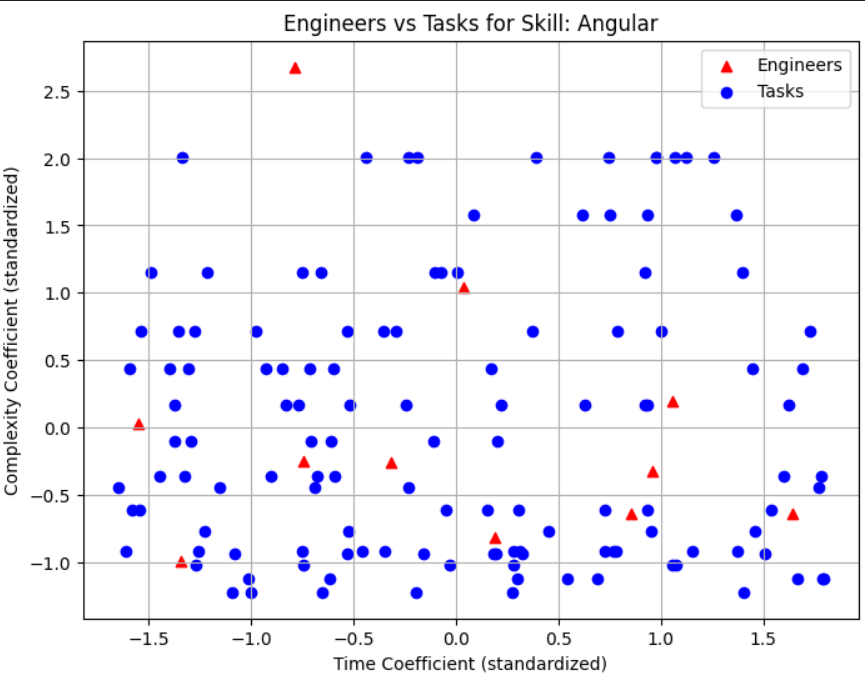
\includegraphics[width=0.9\linewidth]{./figures/all_engineers_tasks.png}
    \caption{Raw task vs engineer vectors: complexity vs time.}
\end{figure}

\begin{figure}[H]
    \centering
    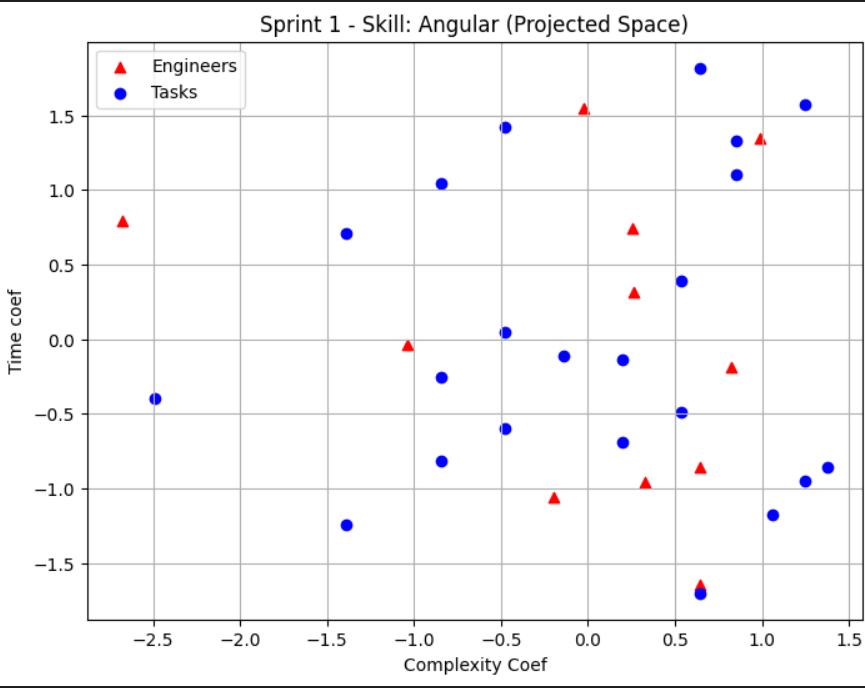
\includegraphics[width=0.9\linewidth]{./figures/projected_space.png}
    \caption{Projected space with eigen-axes and example assignments.}
\end{figure}

\subsection{Quantitative Results}
\begin{table}[H]
    \centering
    \caption{Baseline comparison}
    \begin{tabular}{lcccc}
    \toprule
    Method & Match & Dist & Unassigned & LoadVar \\
    \midrule
    Naive-priority & 0.72 & 2.37 & 28\% & 4.8 \\
    Skill-only     & 0.61 & 3.21 & 39\% & 6.1 \\
    Proposed       & \textbf{0.982} & \textbf{0.852} & \textbf{1.8\%} & \textbf{3.63} \\
    \bottomrule
    \end{tabular}
\end{table}

\begin{table}[H]
    \centering
    \caption{Greedy vs Oracle-Hungarian (OH)}
    \begin{tabular}{lcccc}
    \toprule
    Method & Match & Dist & Unassigned & LoadVar \\
    \midrule
    Greedy & 0.982 & 0.852 & 1.8 & 3.63 \\
    OH--Angular   & 0.639 & 0.511 & 36.1 & 0.0 \\
    OH--React     & 0.871 & 0.623 & 12.9 & 0.0 \\
    \bottomrule
    \end{tabular}
\end{table}

\begin{table}[H]
    \centering
    \caption{Scalability results}
    \begin{tabular}{lcc}
    \toprule
    Tasks & Engineers & Runtime (s) \\
    \midrule
    100  & 50 & 0.018 \\
    500  & 50 & 0.029 \\
    1000 & 50 & 0.035 \\
    \bottomrule
    \end{tabular}
\end{table}

\begin{figure}[H]
    \centering
    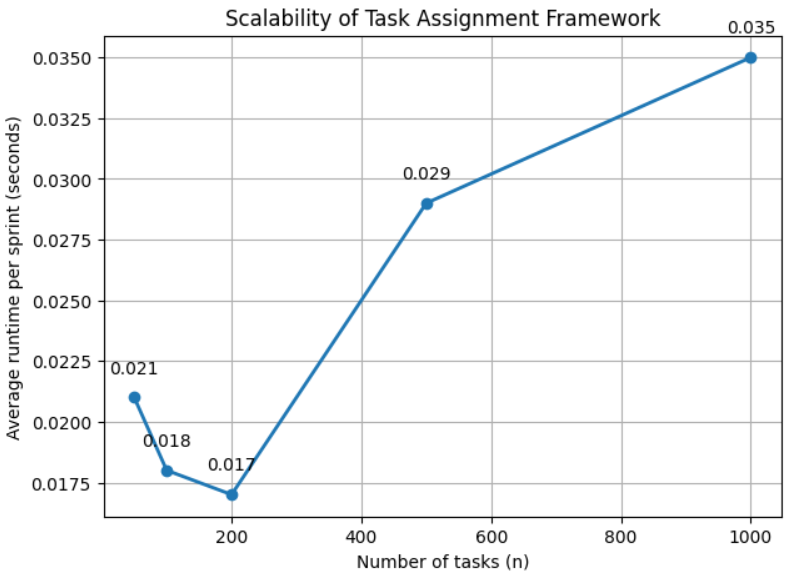
\includegraphics[width=0.9\linewidth]{./figures/complexity_plot.png}
    \caption{Runtime scalability: tasks vs average runtime.}
\end{figure}

% -------------------------------------------------
\section{Discussion and Limitations}
Our framework is interpretable and efficient, producing nearly complete assignments with balanced load. Unlike black-box ML, every assignment is explainable by projected distance. Limitations include reliance on synthetic data, single-skill task modeling, and greedy heuristics rather than global optimization. Future work will validate on industrial datasets, extend to multi-skill tasks, and benchmark against learning-based triage.

% -------------------------------------------------
\section{Conclusion}
We presented a covariance--eigenvector projection framework for sprint-level task allocation. By projecting tasks and engineers into a variance-preserving basis and matching by distance, the method balances transparency, reproducibility, and practical performance. It provides a rigorous baseline for AI-driven allocation research.

\section*{Acknowledgements}
The author thanks Dr.~Lionel Randall Kharkrang, Trieste University, for mentorship, and IIT Patna for academic support.

\section*{Ethics and Conflict of Interest Statement}
The author declares no conflict of interest. Synthetic datasets were used, with no human participants or sensitive data.

% -------------------------------------------------
\begin{thebibliography}{15}

\bibitem{jira_assignment}
JIRA task assignment study, IET Software, 2024.

\bibitem{atlassian_priorities}
Atlassian, ``Issue Priority Field in Jira,'' 2024.

\bibitem{guo2011notmybug}
P. J. Guo, T. Zimmermann, N. Nagappan, and B. Murphy, ``Not my bug!'' ACM CSCW, 2011.

\bibitem{xuan2017bugtriage}
J. Xuan, H. Jiang, Z. Ren, and W. Zou, ``Automatic bug triage,'' IEEE SANER, 2017.

\bibitem{cocomo}
B. W. Boehm, ``COCOMO model overview.''

\bibitem{parametric_estimate}
Motion Inc., ``Parametric estimating,'' 2024.

\bibitem{pca2017}
Tutorial on PCA and eigenvalue methods, arXiv:1701.08106, 2017.

\bibitem{eigen_projection}
T. Zhao, ``Eigen-projection in statistical models.''

\bibitem{bipartite_matching}
Graph matching and task allocation, arXiv:1303.5943, 2013.

\bibitem{BurkardAssignmentBook}
R. E. Burkard, M. Dell’Amico, and S. Martello, \emph{Assignment Problems}. SIAM, 2012.

\bibitem{kuhn1955hungarian}
H. W. Kuhn, ``The Hungarian Method,'' NRLQ, 1955.

\bibitem{munkres1957algorithms}
J. Munkres, ``Algorithms for the assignment problem,'' SIAM J., 1957.

\bibitem{WileyMSPSPReview2018}
C. Brucker, A. Drexl, and R. Klein, ``Multi-skill project scheduling,'' EJOR, 2018.

\bibitem{ReactiveSchedSurvey2006}
A. Ouelhadj and S. Petrovic, ``Dynamic scheduling survey,'' J. Scheduling, 2009.

\bibitem{ribeiro2022xai}
T. L. Ribeiro, M. Singh, and C. G. Andrade, ``Explainable AI in software engineering,'' Empirical SE, 2022.

\end{thebibliography}

\end{document}
